%設定頁面
\documentclass[12pt,a4paper]{article}
\usepackage[margin=1in,a4paper]{geometry}

%設定中文
\usepackage{xeCJK} 
\setCJKmainfont{標楷體} 
\XeTeXlinebreaklocale "zh"   
\XeTeXlinebreakskip = 0pt plus 1pt 

%浮水印
%\usepackage{draftwatermark}
%\SetWatermarkText{\bf NTNU MATH}
%\SetWatermarkScale{0.7}

%圖片
\usepackage{graphicx}
\usepackage{subfigure}

%頁首頁尾
\makeatother
\usepackage{fancyhdr}

%顏色
\usepackage{xcolor}

%表格顏色
\usepackage{colortbl}

%設定數學
\usepackage{amsmath, amsthm, amssymb}
\makeatletter

%自定圈圈標號
\usepackage{pstricks,pstricks-add}
\newcommand\textc[1]{{\begin{pspicture*}
(-0.25,-0.2)(0.25,0.3)\rput[c](0,0)
{\large \textcircled{\footnotesize #1}}
\end{pspicture*} }}

%自訂向量符號
\def\leftharpoonfill@{\arrowfill@\leftharpoonup\relbar\relbar}
\def\rightharpoonfill@{\arrowfill@\relbar\relbar\rightharpoonup}
\newcommand\rbjt{\mathpalette{\overarrow@\rightharpoonfill@}}
\newcommand\lbjt{\mathpalette{\overarrow@\leftharpoonfill@}}

%自訂定理
\newtheorem*{thm}{Theorem}
\newtheorem*{lem}{Lemma}
\newtheorem*{de}{Definition}
\newtheorem*{rmk}{Remark}
\newtheorem*{ex}{Example}
\newtheorem*{pf}{Proof}
\newtheorem*{sol}{Solution}

%程式碼
\usepackage{listings}
\usepackage{color}

\definecolor{dkgreen}{rgb}{0,0.6,0}
\definecolor{gray}{rgb}{0.5,0.5,0.5}
\definecolor{mauve}{rgb}{0.58,0,0.82}

\lstset{
  basicstyle={\small \ttfamily},
  frame=tb,
  language=Python,
  aboveskip=3mm,
  belowskip=3mm,
  showstringspaces=false,
  columns=flexible,
  basicstyle={\small\ttfamily},
  numbers=left,
  numbersep = 14pt,
  numberstyle=\tiny\color{gray},
  keywordstyle=\color{blue},
  commentstyle=\color{dkgreen},
  stringstyle=\color{mauve},
  breaklines=true,
  breakatwhitespace=true,
  tabsize=3,
  backgroundcolor=\color{gray!10}
}




%作者
\title{NTNU影像處理HW6}
\author{廖家緯}
\date{2020.4.21}

\begin{document}
\maketitle
%標題、作者、日期
\fontsize{12pt}{20pt}\selectfont
%設定字體大小、間距
\setlength{\baselineskip}{20pt}
%設定行距

\pagestyle{fancy}
\lhead{}
\chead{}
\rhead{}
\lfoot{}
\cfoot{\thepage}
\rfoot{}
\renewcommand{\headrulewidth}{0pt} %上線寬
\renewcommand{\footrulewidth}{0pt} %下線寬
%\renewcommand{\abstractname}{Executive Summary}




%正文開始
\begin{enumerate}
\item[•]{\bf Outline}:\\
Image Enlargement
\begin{enumerate}
\item[1.]Choose a grayscale image $I$\\
\item[2.]Zero interleave
$I'(i, j) = \begin{cases}
I(\frac{i+1}{2}, \frac{j+1}{2})
& \text{if }i, j:\text{odd}\\
\hspace*{2em}0 & \text{otherwise}
\end{cases}$\\
\item[3.]
Fill values by convolving $I'$ with\\
\begin{enumerate}
\item[(1)]NN interpolation:
$\left[\begin{array}{ccc}
1 & 1 & 0\\
1 & 1 & 0\\
0 & 0 & 0
\end{array}\right]$\\

\item[(2)]Bilinear interpolation:
$\dfrac{1}{4}\left[\begin{array}{ccc}
1 & 2 & 1\\
2 & 4 & 2\\
1 & 2 & 1
\end{array}\right]$\\
\end{enumerate}

\item[4.]Output enlarged images\\
\end{enumerate}

\item[•]
{\bf Code(Python):}
\begin{lstlisting}
# coding: utf-8
import numpy as np
import cv2
    
# Convolution
def conv(Matrix, Filter):
    Matrix = np.pad(Matrix,((1,1),(1,1)),'constant',constant_values = (0,0))
    n, m = np.shape(Matrix)
    Matrix2 = np.zeros((n, m)).astype('double')
    for i in range(1, n-1):
        for j in range(1 ,m-1):
            Matrix2[i,j] =  (Matrix[i-1:i+2, j-1:j+2]*Filter).sum()

    Matrix2 = Matrix2.astype('uint8')
    return Matrix2[1:n-1, 1:m-1]

# Step 1: Choose a grayscale image I
I = cv2.imread('Gray.jpg', cv2.IMREAD_GRAYSCALE)
n, m = np.shape(I)

# Step 2: Zero interleave
I1 = np.zeros((n*2,m*2), np.double)

for i in range(n*2):
    for j in range(m*2):
        if i%2==0 and j%2==0:
            I1[i, j] = I[i//2, j//2]
            
# Step 3: Fill values by convolving I1 with
# (i) NN interpolation
NN = np.array([[1, 1, 0], [1, 1, 0], [0, 0, 0]])

# (ii) Bilinear interpolation
Bilinear = (1/4)*np.array([[1, 2, 1], [2, 4, 2], [1, 2, 1]])

img_NN = conv(I1, NN)
img_Bilinear = conv(I1, Bilinear)

cv2.imwrite('img_NN.jpg', img_NN)
cv2.imwrite('img_Bilinear.jpg', img_Bilinear)

\end{lstlisting}

\item[•]
{\bf Input image:}\\
\begin{figure}[h]
\hspace*{11em}
\begin{tabular}{c}
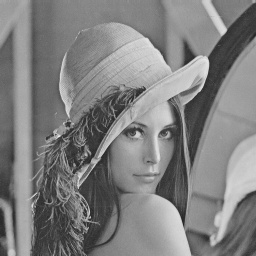
\includegraphics[height=2.4in]{Gray.jpg}\\
Original
\end{tabular}
\end{figure}

\newpage
\item[•]
{\bf Result:}
\begin{figure}[h]
\hspace*{7.5em}
\begin{tabular}{c}
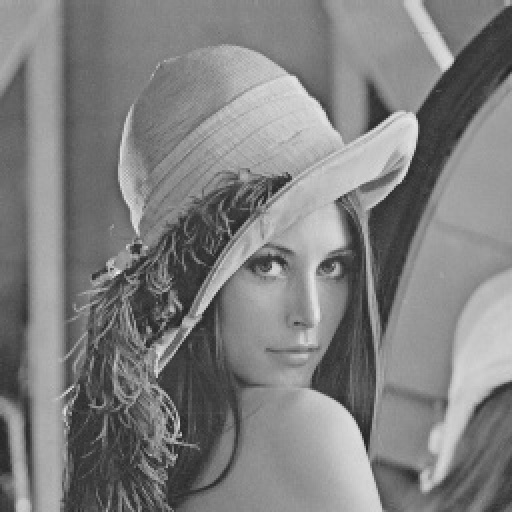
\includegraphics[height=3.5in]{img_NN.jpg}\\
NN \vspace*{0.2em}\\
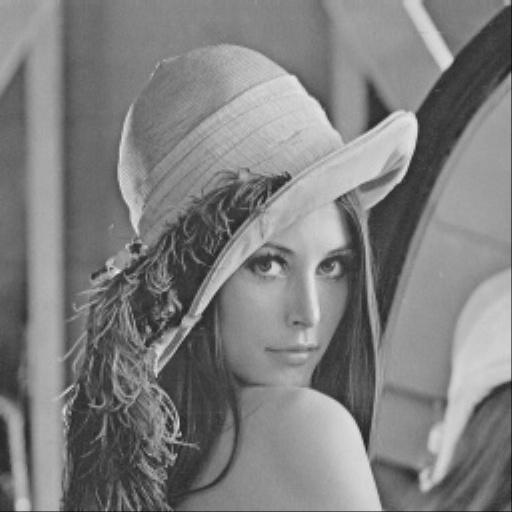
\includegraphics[height=3.5in]{img_Bilinear.jpg}\\
Bilinear
\end{tabular}
\end{figure} 

\newpage
\item[•]
{\bf Experience:}\\
在影像處理中,通常從1開始編號,而我使用的Python程式語言是從0開始編號,因此我的code和老師的步驟有點不同。另外,為了方便對每個pixel做convolution,我在函式中加入padding (補0),做完後再刪去,使得邊界不會產生條紋。
\end{enumerate}










\end{document}